\ifcsname c@none\endcsname\else\newcounter{none}\fi
\subsection{Phạm vi các lượt kiểm thử}
Phần này trình bày phương pháp và kết quả kiểm thử chi tiết TC01--TC06,
kèm ảnh quan sát trên Cisco Packet Tracer. Các ảnh dưới đây
thuộc phiên bản trước khi cập nhật bố trí tầng, camera và SSH; Main-PC10-A
trong các ảnh có IP 10.10.10.8. Ở phiên bản cập nhật, client này nhận
10.10.10.9. Vì địa chỉ DHCP và mô hình có thay đổi, ảnh của lượt trước chỉ
minh chứng lượt thử tương ứng. Các kết quả bổ sung về Wi-Fi, camera và
SSH của mô hình cập nhật được trình bày ở phần sau.

\FloatBarrier
\subsection{Phương pháp kiểm thử kết nối bắt buộc
(Step5)}\label{phux1b0ux1a1ng-phuxe1p-kiux1ec3m-thux1eed-kux1ebft-nux1ed1i-bux1eaft-buux1ed9c-step5}

{\def\LTcaptype{none} % do not increment counter
\begin{longtable}[]{@{}
  >{\raggedright\arraybackslash}p{(\linewidth - 4\tabcolsep) * \real{0.3333}}
  >{\raggedright\arraybackslash}p{(\linewidth - 4\tabcolsep) * \real{0.3333}}
  >{\raggedright\arraybackslash}p{(\linewidth - 4\tabcolsep) * \real{0.3333}}@{}}
\toprule\noalign{}
\begin{minipage}[b]{\linewidth}\raggedright
Ca
\end{minipage} & \begin{minipage}[b]{\linewidth}\raggedright
Thao tác và cặp nguồn--đích đại diện
\end{minipage} & \begin{minipage}[b]{\linewidth}\raggedright
Kỳ vọng và bằng chứng cần đọc
\end{minipage} \\
\midrule\noalign{}
\endhead
\bottomrule\noalign{}
\endlastfoot
TC01 & Ping hai PC trong cùng VLAN, thử hai chiều & Reply sau ARP; xác
nhận mask/VLAN, không suy từ route liên VLAN \\
TC02 & PC khác VLAN và PC tới HIS & Luồng được ACL cho phép thành công;
kiểm gateway và counter \\
TC03 & Main hai chiều DBP và Main hai chiều BHTQ & Hai chiều thành công;
route OSPF/trace đúng đường Main \\
TC04 & Client nội bộ tới DMZ, client ngoài tới ISP2:8080 & HTTP đúng
server; counter firewall/NAT và đường về hợp lệ \\
TC05 & Guest tới PC/HIS, rồi Guest tới Web & Nội bộ thất bại, Internet
thành công; có counter deny và đối chứng \\
TC06 & PC/Guest ba site tới Web bằng IP/tên & HTTP/DNS thành công, PAT
đúng egress tại Main \\
\end{longtable}
}

Ping dùng để kiểm reachability ICMP, traceroute để quan sát các hop khi
nền tảng hỗ trợ, HTTP để kiểm dịch vụ ở lớp ứng dụng, CLI/counter để xác
nhận cơ chế xử lý. Thất bại ping một mình không đủ chứng minh ACL đúng:
có thể do sai IP, mất route hoặc server tắt. Vì vậy ca Guest phải có cả
đối chứng Internet từ cùng client và truy cập HIS từ client được phép.

Các lệnh tái hiện thông thường là ping và tracert trên PC-PT;
kiểm router bằng show ip route, show ip ospf
neighbor, show access-lists và show ip nat translations. Đây là hướng
dẫn thao tác, không phải output thu được. Khi có ARP/DHCP/OSPF warmup,
lưu cả lần đầu và lần thử sau hội tụ thay vì sửa lịch sử thành không
gián đoạn.

\FloatBarrier
\subsection{Kiểm thử chính sách trên Packet Tracer}\label{kiux1ec3m-thux1eed-chuxednh-suxe1ch-vuxe0-kux1ebft-quux1ea3-theo-nux1ec1n-tux1ea3ng}

Khách bị chặn tới mạng nội bộ, server/DMZ, quản trị và camera; vẫn được
DHCP/DNS và Web Internet. Người dùng chỉ được truy cập ứng dụng theo vai
trò; DB không công bố cho client. Camera không được tự truy cập LAN.
Quản trị tập trung từ Main-Admin. Truy cập cùng VLAN cần host
firewall/L2 isolation bổ sung, không được coi ACL gateway đã bảo vệ toàn
bộ east-west.

VPN được đề xuất đủ hai trường hợp theo đề: site-to-site route-based
IPsec/IKEv2 qua leased line; teleworker kết thúc trên firewall, tài
khoản riêng/MFA, split tunnel chỉ tới HIS/CRM được duyệt. Chưa triển
khai crypto, chứng thư, MFA hoặc kiểm MTU; không ghi VPN PASS. Trước
triển khai phải tránh tuyến cleartext ưu tiên hơn tunnel và thêm route
về pool, NAT exemption, ACL/VPN zone.

Sáu nhóm bắt buộc kiểm kết nối cùng VLAN, liên VLAN, liên site, truy cập
DMZ, cách ly Guest và truy cập Web Internet mô phỏng. Các phép kiểm bổ sung
đối chiếu OSPF, DHCP/DNS, NAT, counter ACL và trạng thái sau lưu/mở lại.
Chuyển đường ISP trong Packet Tracer được kiểm bằng thao tác thủ công;
không xem kết quả đó là bằng chứng cân bằng tải hoặc failover tự động.
Internet thật, TLS, RF, GPON PHY, throughput và ứng dụng y tế thực không
nằm trong các phép kiểm này.

\subsubsection{Kết quả Packet Tracer sau mở
lại}\label{kux1ebft-quux1ea3-packet-tracer-sau-mux1edf-lux1ea1i}

{\def\LTcaptype{none} % do not increment counter
\begin{longtable}[]{@{}llr@{}}
\toprule\noalign{}
Nhóm & Phạm vi kiểm & Số lượt \\
\midrule\noalign{}
\endhead
\bottomrule\noalign{}
\endlastfoot
TC01 & Cùng VLAN, hai chiều & 2 \\
TC02 & Liên VLAN và HIS & 3 \\
TC03 & Main với DBP/BHTQ, hai chiều & 4 \\
TC04 & DMZ và static PAT từ ngoài & 2 \\
TC05 & Guest bị chặn LAN/HIS, có đối chứng & 9 \\
TC06 & PC/Guest mỗi site tới Web/DNS & 6 \\
WIFI & Staff mỗi site tới HIS/Web qua Wi-Fi & 6 \\
\end{longtable}
}

Tổng 32 quan sát phù hợp kỳ vọng sau warmup. Tám ping được phép đều nhận
đủ 4/4; ba ping Guest không phản hồi. HTTP cho phép trả đúng URL/nội
dung; HTTP Guest thất bại được đối chiếu với Guest ra Web thành công, PC
nội bộ tới cùng HIS thành công và ACL deny tăng (Main 16, DBP 16, BHTQ
26). Lịch sử lần thử lỗi và warmup được giữ riêng.

Bốn lượt HTTP bổ sung gồm ba nguồn Main-PC10-A, DBP-Guest, BHTQ-Staff
qua ISP1 và một lượt sau khôi phục ISP2; NAT public đúng egress, cấu
hình Edge được khôi phục. Evidence ở
test\_results/packet-tracer/after-reopen/; chạy python
scripts/check\_packet\_runtime.py để kiểm hash và kết quả đã lưu. Phụ
lục packet-tracer-validation.pdf kèm bảng sáu BSSID, IP, SSID và hash
native. Checker offline không chạy lại mạng.

\FloatBarrier
\subsection{Thí nghiệm cụ thể và kết quả Packet Tracer đã
lưu}\label{thuxed-nghiux1ec7m-cux1ee5-thux1ec3-vuxe0-kux1ebft-quux1ea3-packet-tracer-ux111uxe3-lux1b0u}

\subsubsection{TC01: quan sát đầu
cuối}\label{tc01-quan-suxe1t-ux111ux1ea7u-cuux1ed1i}

{\def\LTcaptype{none} % do not increment counter
\begin{longtable}[]{@{}llll@{}}
\toprule\noalign{}
Nguồn & Đích & Giao thức & Kỳ vọng \\
\midrule\noalign{}
\endhead
\bottomrule\noalign{}
\endlastfoot
Main-PC10-A & 10.10.10.7 & ping & allow \\
Main-PC10-B & 10.10.10.8 & ping & allow \\
\end{longtable}
}

\par\Needspace{12\baselineskip}
\noindent\begin{minipage}{\linewidth}
\centering
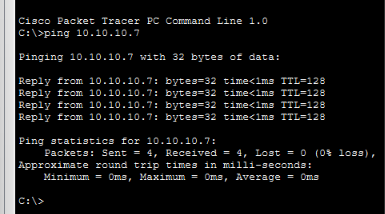
\includegraphics[width=0.85\linewidth,height=\textheight,keepaspectratio,alt={TC01:
Main-PC10-A ping Main-PC10-B (10.10.10.7), nhận đủ 4/4 gói, không mất
gói.}]{assets/tc01-a-to-b.png}
\captionof{figure}{TC01: Main-PC10-A ping Main-PC10-B (10.10.10.7), nhận đủ 4/4
gói, không mất gói.}
\end{minipage}\par\medskip

\par\Needspace{12\baselineskip}
\noindent\begin{minipage}{\linewidth}
\centering
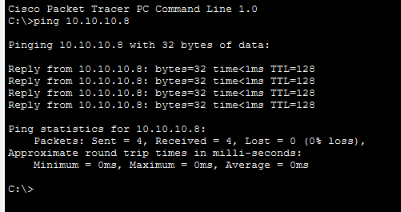
\includegraphics[width=0.85\linewidth,height=\textheight,keepaspectratio,alt={TC01:
Main-PC10-B ping Main-PC10-A (10.10.10.8), nhận đủ 4/4 gói, không mất
gói.}]{assets/tc01-b-to-a.png}
\captionof{figure}{TC01: Main-PC10-B ping Main-PC10-A (10.10.10.8), nhận đủ 4/4
gói, không mất gói.}
\end{minipage}\par\medskip

Kết quả hai chiều cho thấy hai máy trạm trong cùng VLAN10 liên lạc thành
công, với tỷ lệ mất gói 0\% trong mỗi lượt ping.

\subsubsection{TC02: quan sát đầu
cuối}\label{tc02-quan-suxe1t-ux111ux1ea7u-cuux1ed1i}

{\def\LTcaptype{none} % do not increment counter
\begin{longtable}[]{@{}llll@{}}
\toprule\noalign{}
Nguồn & Đích & Giao thức & Kỳ vọng \\
\midrule\noalign{}
\endhead
\bottomrule\noalign{}
\endlastfoot
Main-PC10-A & 10.10.20.7 & ping & allow \\
Main-PC20 & 10.10.10.8 & ping & allow \\
Main-PC10-A & http://10.10.70.11 & http & allow \\
\end{longtable}
}

\par\Needspace{12\baselineskip}
\noindent\begin{minipage}{\linewidth}
\centering
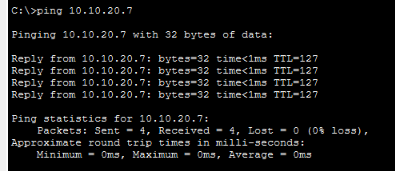
\includegraphics[width=0.85\linewidth,height=\textheight,keepaspectratio,alt={TC02:
Main-PC10-A thuộc VLAN10 ping Main-PC20 (10.10.20.7) thuộc VLAN20, nhận
đủ 4/4 gói, không mất gói.}]{assets/tc02-v10-to-v20.png}
\captionof{figure}{TC02: Main-PC10-A thuộc VLAN10 ping Main-PC20 (10.10.20.7)
thuộc VLAN20, nhận đủ 4/4 gói, không mất gói.}
\end{minipage}\par\medskip

\par\Needspace{12\baselineskip}
\noindent\begin{minipage}{\linewidth}
\centering
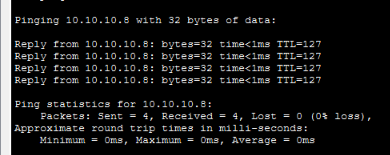
\includegraphics[width=0.85\linewidth,height=\textheight,keepaspectratio,alt={TC02:
Main-PC20 thuộc VLAN20 ping Main-PC10-A (10.10.10.8) thuộc VLAN10, nhận
đủ 4/4 gói, không mất gói.}]{assets/tc02-v20-to-v10.png}
\captionof{figure}{TC02: Main-PC20 thuộc VLAN20 ping Main-PC10-A (10.10.10.8)
thuộc VLAN10, nhận đủ 4/4 gói, không mất gói.}
\end{minipage}\par\medskip

\par\Needspace{12\baselineskip}
\noindent\begin{minipage}{\linewidth}
\centering
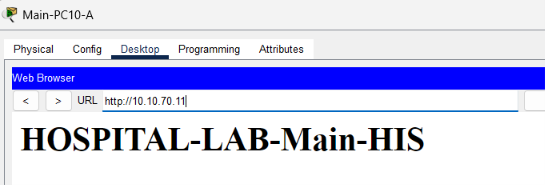
\includegraphics[width=0.85\linewidth,height=\textheight,keepaspectratio,alt={TC02:
Main-PC10-A truy cập http://10.10.70.11 và nhận trang
HOSPITAL-LAB-Main-HIS.}]{assets/tc02-his-http.png}
\captionof{figure}{TC02: Main-PC10-A truy cập http://10.10.70.11 và nhận trang
HOSPITAL-LAB-Main-HIS.}
\end{minipage}\par\medskip

Kết quả ping hai chiều cho thấy kết nối được phép giữa VLAN10 và VLAN20
hoạt động, với tỷ lệ mất gói 0\% trong mỗi lượt. Trình duyệt trên
Main-PC10-A hiển thị trang HOSPITAL-LAB-Main-HIS tại địa chỉ
10.10.70.11, minh chứng máy trạm VLAN10 truy cập được dịch vụ HTTP đại
diện HIS trong VLAN70.

\clearpage

\subsubsection{TC03: quan sát đầu
cuối}\label{tc03-quan-suxe1t-ux111ux1ea7u-cuux1ed1i}

{\def\LTcaptype{none} % do not increment counter
\begin{longtable}[]{@{}llll@{}}
\toprule\noalign{}
Nguồn & Đích & Giao thức & Kỳ vọng \\
\midrule\noalign{}
\endhead
\bottomrule\noalign{}
\endlastfoot
Main-PC10-A & 10.20.10.7 & ping & allow \\
DBP-PC10 & 10.10.10.8 & ping & allow \\
Main-PC10-A & 10.30.10.7 & ping & allow \\
BHTQ-PC10 & 10.10.10.8 & ping & allow \\
\end{longtable}
}

\par\Needspace{12\baselineskip}
\noindent\begin{minipage}{\linewidth}
\centering
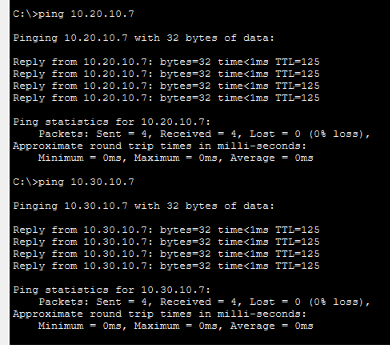
\includegraphics[width=0.85\linewidth,height=\textheight,keepaspectratio,alt={TC03:
từ Main ping DBP-PC10 (10.20.10.7) và BHTQ-PC10 (10.30.10.7); mỗi lượt
nhận đủ 4/4 gói, tỷ lệ mất gói 0\%.}]{assets/tc03-main-to-aux.png}
\captionof{figure}{TC03: từ Main ping DBP-PC10 (10.20.10.7) và BHTQ-PC10
(10.30.10.7); mỗi lượt nhận đủ 4/4 gói, tỷ lệ mất gói 0\%.}
\end{minipage}\par\medskip

Ảnh minh chứng kết nối từ Main tới cả hai cơ sở phụ DBP và BHTQ. Hai
lượt ping đều nhận đủ bốn gói phản hồi, cho thấy đường đi và đường trả
lời ICMP giữa Main với từng cơ sở phụ hoạt động. Các lượt khởi tạo ping
từ DBP/BHTQ về Main trong bảng được ghi nhận riêng trong hồ sơ kiểm thử.

\clearpage

\subsubsection{TC04: quan sát đầu
cuối}\label{tc04-quan-suxe1t-ux111ux1ea7u-cuux1ed1i}

{\def\LTcaptype{none} % do not increment counter
\begin{longtable}[]{@{}llll@{}}
\toprule\noalign{}
Nguồn & Đích & Giao thức & Kỳ vọng \\
\midrule\noalign{}
\endhead
\bottomrule\noalign{}
\endlastfoot
Main-PC10-A & http://10.10.80.10 & http & allow \\
Web-Lab & http://198.51.100.2:8080 & http & allow \\
\end{longtable}
}

\par\Needspace{12\baselineskip}
\noindent\begin{minipage}{\linewidth}
\centering
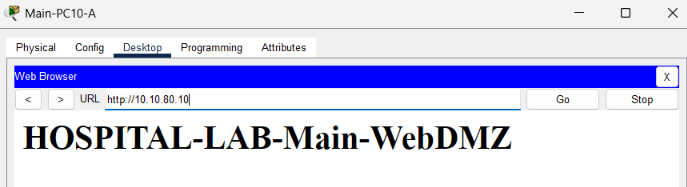
\includegraphics[width=0.85\linewidth,height=\textheight,keepaspectratio,alt={TC04:
Main-PC10-A truy cập http://10.10.80.10 và nhận trang
HOSPITAL-LAB-Main-WebDMZ.}]{assets/tc04-internal-webdmz.png}
\captionof{figure}{TC04: Main-PC10-A truy cập http://10.10.80.10 và nhận trang
HOSPITAL-LAB-Main-WebDMZ.}
\end{minipage}\par\medskip

\par\Needspace{12\baselineskip}
\noindent\begin{minipage}{\linewidth}
\centering
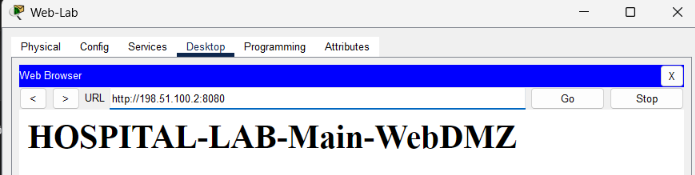
\includegraphics[width=0.85\linewidth,height=\textheight,keepaspectratio,alt={TC04:
Web-Lab truy cập http://198.51.100.2:8080 và nhận trang
HOSPITAL-LAB-Main-WebDMZ.}]{assets/tc04-external-webdmz.png}
\captionof{figure}{TC04: Web-Lab truy cập http://198.51.100.2:8080 và nhận trang
HOSPITAL-LAB-Main-WebDMZ.}
\end{minipage}\par\medskip

Trình duyệt trên Main-PC10-A hiển thị trang HOSPITAL-LAB-Main-WebDMZ tại
địa chỉ 10.10.80.10, minh chứng máy trạm nội bộ truy cập được dịch vụ
HTTP của server trong vùng DMZ. Từ phía ngoài, Web-Lab mở địa chỉ công
bố 198.51.100.2:8080 và nhận cùng trang WebDMZ. Kết quả này phù hợp với
cấu hình static PAT chuyển tiếp cổng 8080 trên địa chỉ ngoài của
Main-Edge phía ISP2 tới cổng HTTP 80 của server 10.10.80.10.

\clearpage

\subsubsection{TC05: quan sát đầu
cuối}\label{tc05-quan-suxe1t-ux111ux1ea7u-cuux1ed1i}

{\def\LTcaptype{none} % do not increment counter
\begin{longtable}[]{@{}llll@{}}
\toprule\noalign{}
Nguồn & Đích & Giao thức & Kỳ vọng \\
\midrule\noalign{}
\endhead
\bottomrule\noalign{}
\endlastfoot
Main-Guest & 10.10.10.8 & ping & deny \\
Main-PC10-A & http://10.10.70.11 & http & allow \\
Main-Guest & http://10.10.70.11 & http & deny \\
DBP-Guest & 10.20.10.7 & ping & deny \\
DBP-PC10 & http://10.10.70.11 & http & allow \\
DBP-Guest & http://10.10.70.11 & http & deny \\
BHTQ-Guest & 10.30.10.7 & ping & deny \\
BHTQ-PC10 & http://10.10.70.11 & http & allow \\
BHTQ-Guest & http://10.10.70.11 & http & deny \\
\end{longtable}
}

\par\Needspace{12\baselineskip}
\noindent\begin{minipage}{\linewidth}
\centering
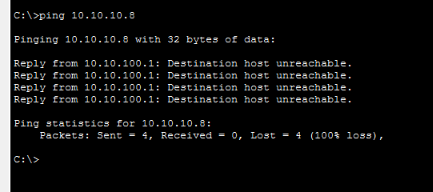
\includegraphics[width=0.8\linewidth,height=\textheight,keepaspectratio,alt={TC05:
Guest ping PC nội bộ 10.10.10.8 không thành công; gateway 10.10.100.1
trả Destination host unreachable, không nhận được gói Echo Reply từ
đích.}]{assets/tc05-guest-ping-denied.png}
\captionof{figure}{TC05: Guest ping PC nội bộ 10.10.10.8 không thành công; gateway
10.10.100.1 trả Destination host unreachable, không nhận được gói Echo
Reply từ đích.}
\end{minipage}\par\medskip

\par\Needspace{12\baselineskip}
\noindent\begin{minipage}{\linewidth}
\centering
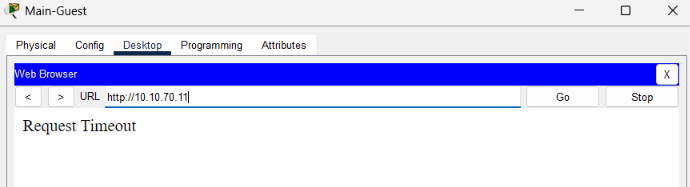
\includegraphics[width=0.85\linewidth,height=\textheight,keepaspectratio,alt={TC05:
Main-Guest truy cập HIS tại http://10.10.70.11 nhận Request
Timeout.}]{assets/tc05-guest-his-denied.png}
\captionof{figure}{TC05: Main-Guest truy cập HIS tại http://10.10.70.11 nhận
Request Timeout.}
\end{minipage}\par\medskip

Hai ảnh ghi nhận Guest không liên lạc được với PC nội bộ và không mở
được dịch vụ HIS. Ảnh truy cập HIS từ Main-PC10-A ở TC02 là đối chứng
cho thấy dịch vụ này hoạt động từ nguồn được phép. Việc xác định gói bị
ACL chặn cần đối chiếu thêm cấu hình và counter, không chỉ dựa vào thông
báo timeout.

\clearpage

\subsubsection*{Đối chứng: Guest vẫn truy cập được
Web-Lab}\label{ux111ux1ed1i-chux1ee9ng-guest-vux1eabn-truy-cux1eadp-ux111ux1b0ux1ee3c-web-lab}

\par\Needspace{12\baselineskip}
\noindent\begin{minipage}{\linewidth}
\centering
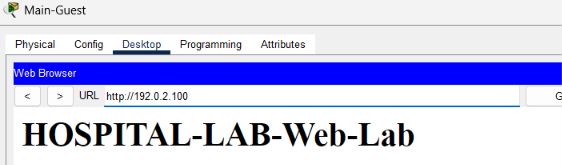
\includegraphics[width=0.85\linewidth,height=\textheight,keepaspectratio,alt={TC05:
Main-Guest mở http://192.0.2.100 và nhận trang
HOSPITAL-LAB-Web-Lab.}]{assets/tc05-guest-web-ip.png}
\captionof{figure}{TC05: Main-Guest mở http://192.0.2.100 và nhận trang
HOSPITAL-LAB-Web-Lab.}
\end{minipage}\par\medskip

\par\Needspace{12\baselineskip}
\noindent\begin{minipage}{\linewidth}
\centering
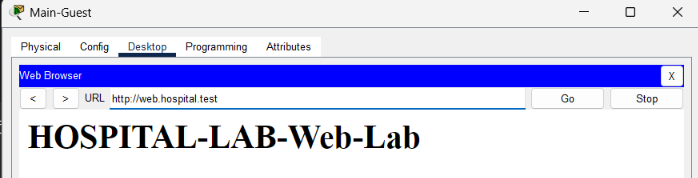
\includegraphics[width=0.85\linewidth,height=\textheight,keepaspectratio,alt={TC05:
Main-Guest mở http://web.hospital.test và nhận trang
HOSPITAL-LAB-Web-Lab.}]{assets/tc05-guest-web-dns.png}
\captionof{figure}{TC05: Main-Guest mở http://web.hospital.test và nhận trang
HOSPITAL-LAB-Web-Lab.}
\end{minipage}\par\medskip

Main-Guest vẫn truy cập được Web-Lab bằng cả địa chỉ IP và tên miền. Hai
kết quả đối chứng cho thấy kết nối HTTP ra mạng Internet mô phỏng và
phân giải tên phục vụ lượt truy cập này hoạt động. Kết hợp với các thử
nghiệm bị từ chối phía trên, kết quả phù hợp chính sách cách ly Guest
khỏi mạng nghiệp vụ nhưng vẫn cho phép truy cập Web bên ngoài. Các ảnh
minh chứng tại Main; kết quả DBP và BHTQ trong bảng được ghi nhận riêng
trong hồ sơ kiểm thử.

\clearpage

\subsubsection{TC06: quan sát đầu
cuối}\label{tc06-quan-suxe1t-ux111ux1ea7u-cuux1ed1i}

{\def\LTcaptype{none} % do not increment counter
\begin{longtable}[]{@{}llll@{}}
\toprule\noalign{}
Nguồn & Đích & Giao thức & Kỳ vọng \\
\midrule\noalign{}
\endhead
\bottomrule\noalign{}
\endlastfoot
Main-PC10-A & http://web.hospital.test & http & allow \\
Main-Guest & http://web.hospital.test & http & allow \\
DBP-PC10 & http://web.hospital.test & http & allow \\
DBP-Guest & http://web.hospital.test & http & allow \\
BHTQ-PC10 & http://web.hospital.test & http & allow \\
BHTQ-Guest & http://web.hospital.test & http & allow \\
\end{longtable}
}

Các quan sát thuộc lần kiểm sau mở lại ngày 04/11/2026. Bảng là bản
trình bày evidence đã lưu; hồ sơ chưa có ảnh chụp giao diện cho từng ca.

\FloatBarrier
\FloatBarrier
\clearpage
